\documentclass{article}
\usepackage{graphicx}
\begin{document}
\newcommand {\GTK}{\textbf{GTK}}
\newcommand {\nItem}[1]{\item{ \(\underline{#1}\)}}

\newpage
\title{Multi-Agent System Simulator\\Software Requirements Specification }
\author{Boch Mike, Gotthold Benjamin, Sharma Varun, Zimmerman Stefan\\
         CISC 475-675 \\
         University of Delaware,\\
         Newark, USA\\}
\date{\today}
\maketitle

\newpage
\tableofcontents

\newpage
\section{Introduction}

The idea of a generic multi agent simulator is not new, however no such platforms exist in the public domain. This platform will construct a simulation environment based on a user generated file adhering to a specific grammar. After creating a simulation, our platform will allow any number of user defined software agents to connect before running a simulation in accordance with the users input. Upon completion of the simulation, our system will produce an easy to read output that highlights key statistics as well as a through log of all events that occurred inside the simulation.

\subsection{Purpose}

The purpose of this Software Requirements Specification (SRS) is to serve as a statement of understanding between the users of the proposed product and the software developers of the product. The software requirements specification is defined using a subset of the Unified Modeling Language, an Entity-Relation diagram describing all of the objects/entities along with their attributes, relations, and Data Flow Diagram (DFD).

\subsection{Scope}

The scope of the system is to develop a general-purpose simulator for Multi-Agent Systems (MAS) and investigate how things play out when agents are given particular algorithms to achieve their goals. This system will run inside a bash script based GUI that takes as input a syntactically correct cTAEMS file containing the simulation parameters. The platform must support the three most basic cTAEMS operations, \textit{and}, \textit{or}, and \textit{sum} when reading in tasks, subtasks, and methods to be executed during runtime. When running, the program will have a predefined window in which user defined software agents can connect through a socket and join the simulation. While running, the simulation allows inter-agent communication and logs statistics related to the number of messages sent by each agent.  Upon completion of a task the system will output an easy to read file containing these statistics as well information related to the quality, cost, and duration of the simulation. The output will also contain a log detailing all events and actions that took place during the run.

It is important to note that this SRS document only pertains to the requirements of the software of a general-purpose simulator for multi-agent systems. It does not include requirements for the designing any particular agents.  The requirements and implementation of the user defined agents, is outside the scope of this document and is therefore not included. 

\subsection{Acronyms and Abbreviations}

This section contains definitions of technical terms and phrases used in this document. Acronyms and abbreviations also appear in this section:

\begin{enumerate}
\item{MAS: Multi-Agent Systems}
\item{UML : Unified Modeling Language}
\item{DFD: Data Flow Diagram}
\item{TCP : Transmission Control Protocol}
\item{SRS: Software Requirements Specification}
\item{GUI: Graphical User Interface}
\item{NLE: Non-local effects}
\item{QAF: Quality Accumulation Function}
\end{enumerate}

\newpage
\section{General Description}
The product is meant to serve as a common platform for academic and research oriented activities in the area of multi-agent simulation. The following sections describe the high level view of the system and establish its context. These sections do not state specific requirements but make the specific requirements easier to understand.

\subsection{Stakeholders}
The users of the Multi-Agent System Simulator are classified into the following categories:

\begin{itemize}
\item{\textbf{Dr. Decker}: Needs a platform to test his software agents in a way that can help advance his research and lead to new innovations.}

\item{\textbf{Dr. Siegel}: Needs a challenging project for his 475 students that is able to be completed over the course of the semester. The project should condone the use of software tools to test implementations and  track changes.}

\item{\textbf{Researchers}: Researchers might want to use this software for their research or design agents and simulations when testing new ideas.}

\item{\textbf{CIS faculty}: Needs an interactive tool for students to make the task of learning more interesting.}

\item{\textbf{Developer}: Developers are responsible for the designing, testing, configuring, and upgrading of subsystem.}

\item{\textbf{Support}: Support personnel are responsible for the maintenance of the system, software, as well as the installation of subsystems and configuration changes.}
\end{itemize}

\subsection{Definition of concepts}
\begin{itemize}
\item{\textbf{Agent}: A user defined software program that can communicate with the simulation through a TCP socket connection.}

\item{\textbf{Multi-agent System}: A Project that includes two or more independent software agents working to complete a common goal}

\item{\textbf{cTEMS}: A derivative of the TAEMS language that will be employed for specifying task domains.}

\item{\textbf{And}: The logical AND where all operands involved in the operation must be true.}

\item{\textbf{Or}: The logical OR where at least one operand involved in the operation must be true.}

\item{\textbf{Sum}: The amount resulting in the addition of two or more operands.}

\item{\textbf{Socket}: The terminating point of a connection across a network used to exchange data.}

\item{\textbf{Bash Script}:  A computer program designed to run inside of a unix system.}

\item{\textbf{Quality}: A user defined numeric value used to measure the degree of satisfaction resulting from a particular event.}

\item{\textbf{Quality Accumulation Function}: QAF is used to compute the quality of tasks (and ultimately overall quality) for a specific execution trace.}

\item{\textbf{Cost}: A user defined numeric value used to measure the resources consumed as a result of a particular event.}

\item{\textbf{Task Group}: A high level grouping of tasks that share a similar structure or goal.}

\item{\textbf{Task}: A high level goal within the system.}

\item{\textbf{Subtask}: A low level goal required to complete a task.}

\item{\textbf{Method}: An action taken in order to complete a task or subtask.}

\item{\textbf{Tick}: A one unit advancement of an internal counter used as a clock.}
\end{itemize}

\newpage
\section{General System Design}

The Multi-Agent Simulator is designed as a central process; all agents involved with the model are connected to the simulator using sockets. The agents themselves are independent processes, which could run on physically different machines. The simulator controls all time synchronization activities, by periodically sending ticks  to each of its remote agents. The simulator is also a message router, where all agent communications will pass through it. This scheme permits explicit control over network and communication delays.

\subsection{System Features}

The following list offers a brief outline and description of the main features and functionalities of the Multi-Agent System Simulator. The features are split into two major categories: core features and additional features. Core features are essential to the application's operation, whereas additional features simply add new functionalities. The latter features will only be implemented as time permits.
\begin{center} Core Features \end{center}

\begin{itemize}
\item{\textbf{CTEAMS file} : The system will read in a file and check that it adheres to the correct syntactical structure. If there is an error in the file, the system will report where it found the error and what the problem was. The System is only required to support the use of the AND, OR, and SUM logical functions of the cTEAMS grammar. After reading in the file, the system will construct a simulation environment and explore all possible outcomes of the simulation.}

\item{\textbf{Config file} : The program will look for a configuration file containing information such as the random number seed. If no configuration file is found the system will make one with default values.}

\item{\textbf{Synchronization clock} : The synchronization clock is located centrally at the simulation controller. It is discrete and pulse ${/}$ tick based. During each cycle a pulse is sent to each attached agent, upon completion, each agent responds to the simulator.}

\item{\textbf{Stats} : The system will produce an easy to read output containing statistics which include the number of messages passed by each agent, the time it took the simulation to complete and the resulting quality and cost of tasks that were attempted by the system.}

\item{\textbf{Logs} : The system will output a detailed log file including the intermediate cost and quality between every method as well as a transcript of agent communication.}

\item{\textbf{Agent Interface} : The system will provide a consistent interface of which all agents must implement in order to connect to the internal communication model. The system must handle any agent architecture in compliance with the Agent Interface and simulation structure and refuse connection to any agent in violation of these elements.}

\item{\textbf{Communications Module} : All communication between the agents and the simulator is controlled by the communication module.  This module also allows an agent to broadcast a message to all other agents without explicitly knowing the number of agents that will receive the message.}

\item{\textbf{Event Engine} :The simulator behavior is directed by a queue containing a time-ordered list of events. Each message it receives either adds or removes events from the queue. At each pulse the simulator selects the correct events and realizes their effects.}

\end{itemize}

\begin{center} Additional Features \end{center}

\begin{itemize}

\item{\textbf{Graphical Representation of Task Structure} : A task structure is a hierarchical tree-like structure representing the Task, Methods, Quality Accumulation Function, Method Interrelationship and resources. We would like to represent this structure as a graphical model to help understand the simulation results better.}

\item{\textbf{Debugging and error handling in cTAEMS or config files} : Log files should locate the point of failure in a buggy cTAEMS or config file. Debugging feature can also be added for handling faulty config and cTAEMS files.}

\item{\textbf{cTEAMS  grammar support} : The system may go beyond the logical AND, OR, and SUM operations and include additional implementations within the cTEAMS grammar.}

\item{\textbf{Agent Behavior} : The System may optionally support the ability of agents to stop, pause, or resume tasks if such actions are applicable based on the simulation specifications. }

\end{itemize}

\newpage
\section{Other non-functional requirements}

\subsection{Performance requirements}

All agents involved with the model are connected to the simulator using sockets. The agents themselves are independent processes, which could run on physically different machines. Note that the simulator does not control the agents' activities, it merely allocates time slices and records the activities performed by the agent during the time slice. This makes the performance of the simulator independent of the agents performance. The performance of the simulator can be affected by the number of socket connections. The system shall function in real-time the effect of network load or maximum limit on socket connections can only be published after testing.

\subsection{Maintainability}

The standardized design and implementation documents will be provided in order to maintain the system. All changes will be documented. A standard architecture will be applied and therefore allowing for quick evolution of the software to adapt to possible situations in the future.

\subsection{Software Quality Attributes}

The user interface of the Multi-Agent System Simulator is to be designed with usability as the first priority. The system will be presented and organized in a manner that is both visually appealing and easy for the user to navigate. To ensure reliability and correctness, there will be zero tolerance for errors in the simulator environment. 

\newpage
\section{Detail System Description}

A Multi-Agent Simulator is domain independent, all domain knowledge is obtained either from configuration files or data received from agents working in the environment. Agents running in the MASS environment use cTAMES a domain-independent, hierarchical representation of the agent's goals, to represent their knowledge. To prevent any interference or assumption, the simulator and the agents run as separate processes. The cTAMES model supplies the internal knowledge of the simulator manager. This coupled with the easy configuration mechanism, logging, reporting and statistical analysis makes the simulator a good platform  for research and evaluation of Multi-Agent Systems.

On initializing the simulator, it reads the configuration and uses them to instantiate other sub-systems in the system. The most vital piece of data originating from the agent is the global task view which is built at the simulator. This global objective view will be used by the execution subsystem when the simulation is running to quantify  both the characteristics of method execution and the effects interactions with resources and other actions have on that method. The event engine manages the queue of events which represent the actions that are taking place. The communications module, maintains a TCP stream connection with each agent, and is responsible for routing the different kinds of messages between the agents and destinations within the simulator. Figure 1 shows a general architecture of the Multi-Agent System Simulator.

\begin{figure}
\centering
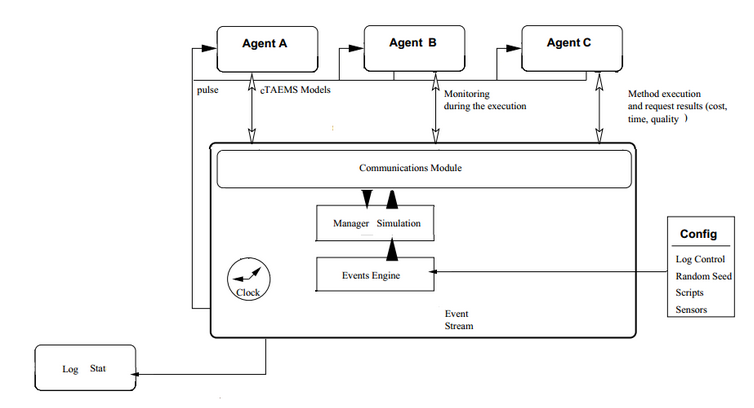
\includegraphics[width=4.5in]{fig1}
\caption{Detail Architecture}
\label{fig_sim}
\end{figure}


\subsection{Sequence Diagram}

Figure 2. represents an event-sequence diagram showing how the services interact with each other for the Multi-Agent System Simulator. 

\begin{figure}
\centering
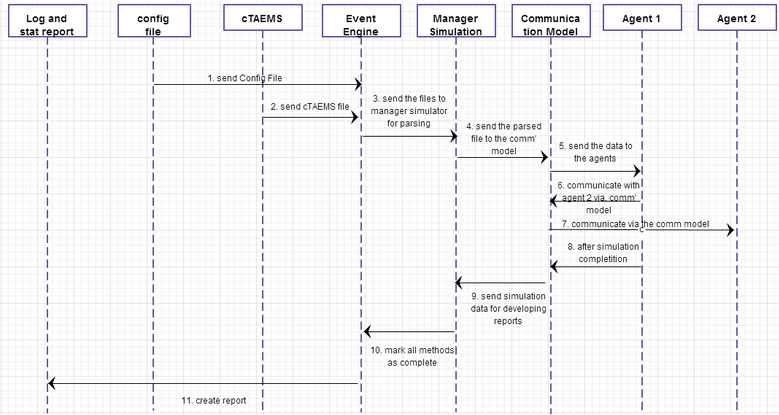
\includegraphics[width=6.0in]{fig2}
\caption{Sequence Diagram}
\label{fig_sim}
\end{figure}

\newpage
\subsection{Data Flow Diagram}

Figure 3. represents the data flow diagram for the entire system.

\begin{figure}[!]
\centering
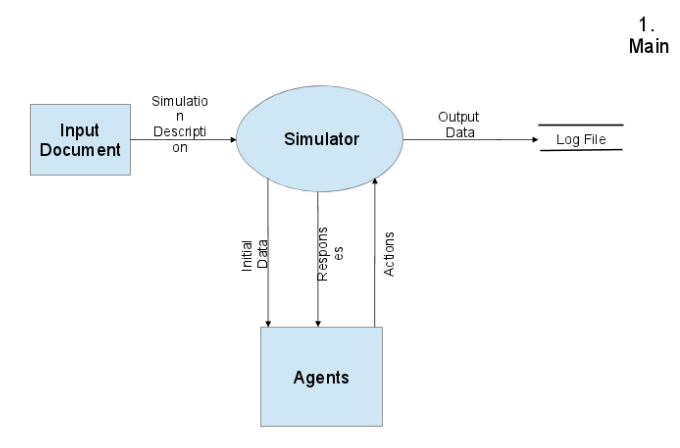
\includegraphics[width=4.0in]{fig3}
\caption{Data Flow Diagram (Level 0)}
\label{fig_sim}
\end{figure}
\newpage

\begin{figure}[!]
\centering
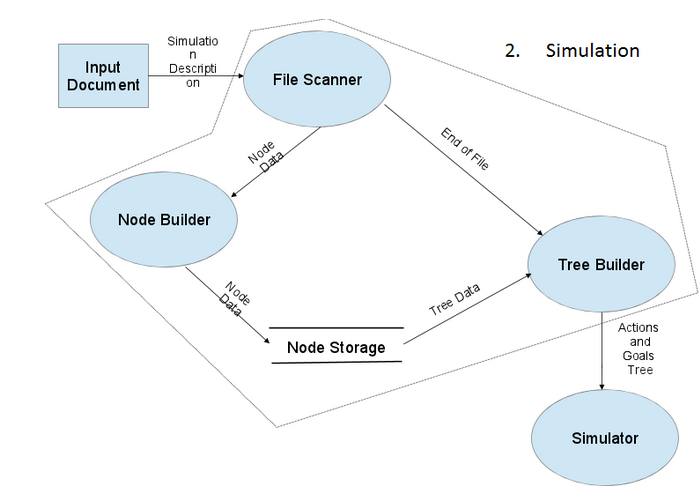
\includegraphics[width=4.0in]{fig4}
\caption{Data Flow Diagram (Level 1)}
\label{fig_sim}
\end{figure}
\newpage

\begin{figure}[!]
\centering
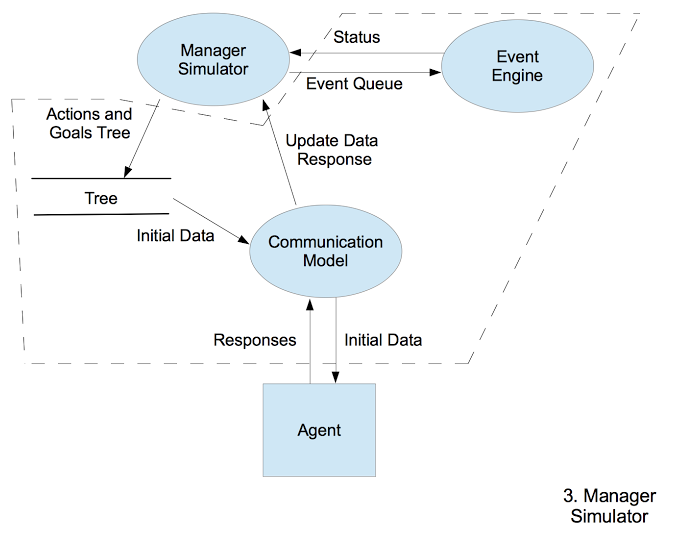
\includegraphics[width=4.0in]{fig5}
\caption{Data Flow Diagram (Level 2)}
\label{fig_sim}
\end{figure}

\begin{figure}[!]
\centering
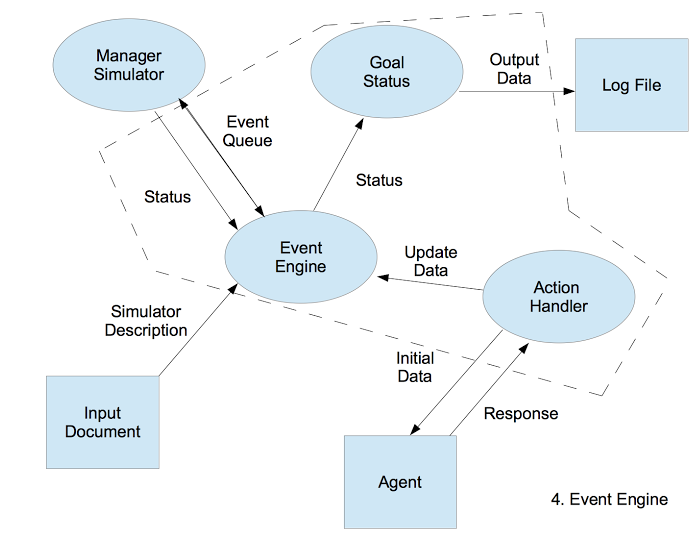
\includegraphics[width=4.0in]{fig6}
\caption{Data Flow Diagram (Level 3)}
\label{fig_sim}
\end{figure}


\newpage 
\section{Conclusion}
Overall, a comprehensive list of requirements has been created. Due to the explorative and innovative character of the project, it is rather a broad and deep insight in the examined area of Multi-Agent System Simulator. Thus, it should facilitate further focusing on project aims and guide to successful case studies and prototypes. The latter will be used to identify new or still overseen demands.

\end{document}
